\documentclass[12pt]{article}
\usepackage[margin=0.8in]{geometry}
\usepackage{xcolor}
\usepackage{enumitem}
\usepackage{tikz}
\usepackage{fancyvrb}
\usetikzlibrary{shapes,arrows,positioning}

% Define placeholder command for variables
\newcommand{\var}[1]{\textcolor{blue}{\texttt{[#1]}}}
\newcommand{\bold}[1]{\textbf{#1}}
\newcommand{\cond}[1]{\textcolor{red}{\texttt{#1}}}

% Style for flowchart
\tikzstyle{decision} = [diamond, draw, fill=blue!20, text width=4.5em, text badly centered, node distance=3cm, inner sep=0pt]
\tikzstyle{block} = [rectangle, draw, fill=blue!20, text width=5em, text centered, rounded corners, minimum height=4em]
\tikzstyle{line} = [draw, -latex']

\title{Trade Narrative Templates for Copy Editing}
\author{TCPT Application}
\date{\today}

\begin{document}

\maketitle

\section*{Instructions}
This document contains the text templates for all narrative generators in the trade application. Variables are shown in \var{blue monospace} format. The actual application replaces these with dynamic content based on the selected country and data.

\section{Trade Overview Narrative (generateTradeNarrative)}

\subsection{Example Output}
\begin{quote}
\textit{As of 2024, \textbf{China} ranked 3\textsuperscript{rd} among all \textbf{U.S.} trading partners by total goods trade — up from 6\textsuperscript{th}. It is currently the 1\textsuperscript{st} largest source of imports and the 3\textsuperscript{rd} largest destination for exports.}

\textit{While the \textbf{U.S.} currently runs a trade deficit with \textbf{China}, this has not always been the case. Over the past 32 years, the \textbf{U.S.} has run a deficit in 78\% of years. This trend has strengthened in recent years, with the \textbf{U.S.} running a deficit in 4 out of 5 years over the past 5 years.}

\textit{\textbf{China} accounts for 16.2\% of total \textbf{U.S.} imports (\$427.2B) and 8.7\% of \textbf{U.S.} exports (\$147.8B), resulting in a deficit of \$279.4B.}
\end{quote}

\subsection{Basic Trade Ranking (Always Shown)}
As of \var{latestYear}, \bold{\var{countryName}} ranked \var{tradeRank\_latest} among all \bold{U.S.} trading partners by total goods trade — \var{tradeDirection}. It is currently the \var{importRank\_latest} largest source of imports and the \var{exportRank\_latest} largest destination for exports.

\subsection{Trade Balance Decision Flow}

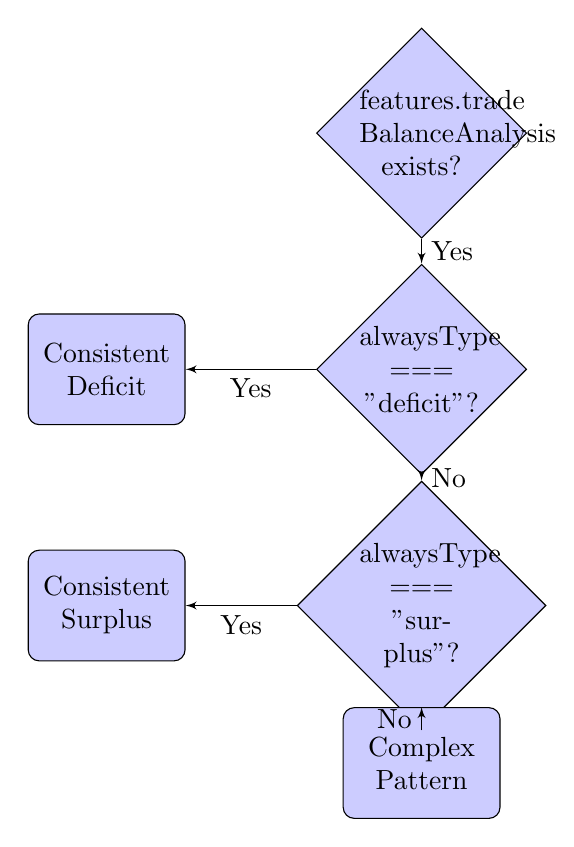
\begin{tikzpicture}[node distance = 2cm, auto]
\node [decision] (check) {features.trade\\BalanceAnalysis exists?};
\node [decision, below of=check] (always) {alwaysType === "deficit"?};
\node [block, left of=always, xshift=-2cm] (deficit) {Consistent Deficit};
\node [decision, below of=always] (surplus) {alwaysType === "surplus"?};
\node [block, left of=surplus, xshift=-2cm] (surplusblock) {Consistent Surplus};
\node [block, below of=surplus] (complex) {Complex Pattern};

\path [line] (check) -- node {Yes} (always);
\path [line] (always) -- node {Yes} (deficit);
\path [line] (always) -- node {No} (surplus);
\path [line] (surplus) -- node {Yes} (surplusblock);
\path [line] (surplus) -- node {No} (complex);
\end{tikzpicture}

\subsection{Trade Balance Scenarios}

\subsubsection{Consistent Deficit}
\textbf{Condition:} \cond{alwaysType === "deficit"}

The \bold{U.S.} has consistently run a trade deficit with \bold{\var{countryName}} since 1992.

\subsubsection{Consistent Surplus}
\textbf{Condition:} \cond{alwaysType === "surplus"}

The \bold{U.S.} has consistently maintained a trade surplus with \bold{\var{countryName}} since 1992.

\subsubsection{Complex Alternating Pattern}
\textbf{Condition:} \cond{alwaysType is neither "deficit" nor "surplus"}

While the \bold{U.S.} currently runs a trade \var{currentStatusText} with \bold{\var{countryName}}, this has not always been the case. Over the past \var{totalYearsAnalyzed} years, the \bold{U.S.} has run a \var{currentStatusText} in \var{currentPercentage}\% of years.

\paragraph{Pattern Stability Logic:}
The pattern stability is determined by comparing historical rates vs. recent 5-year rates using \cond{rateDifference = |recentRate - historicalRate|}:

\begin{itemize}[noitemsep]
\item \textit{Stable pattern:} \cond{rateDifference < 0.2 AND recent5yrPct is between 1-99\%}\\
``This pattern has not changed substantially in recent years, with the \bold{U.S.} running a \var{currentStatusText} in \var{recent5yrYears} out of \var{yearsAnalyzed5yr} years over the past 5 years.''

\item \textit{Intensified pattern:} \cond{recentRate > historicalRate AND recent5yrPct === 100\%}\\
``This trend has intensified in recent years, with the \bold{U.S.} running a \var{currentStatusText} in every year over the past 5 years.''

\item \textit{Strengthened pattern:} \cond{recentRate > historicalRate AND recent5yrPct < 100\%}\\
``This trend has strengthened in recent years, with the \bold{U.S.} running a \var{currentStatusText} in \var{recent5yrYears} out of \var{yearsAnalyzed5yr} years over the past 5 years.''

\item \textit{Weakened pattern:} \cond{recentRate < historicalRate AND recent5yrPct > 0\%}\\
``However, this pattern has weakened in recent years, with the \bold{U.S.} running a \var{currentStatusText} in only \var{recent5yrYears} out of \var{yearsAnalyzed5yr} years over the past 5 years.''

\item \textit{Reversed pattern:} \cond{recentRate < historicalRate AND recent5yrPct === 0\%}\\
``However, this pattern has reversed in recent years, with the \bold{U.S.} running no \var{currentStatusText} in the past 5 years.''
\end{itemize}

\subsection{Trade Values Summary}
\bold{\var{countryName}} accounts for \var{importShare}\% of total \bold{U.S.} imports (\var{importValue}) and \var{exportShare}\% of \bold{U.S.} exports (\var{exportValue}), resulting in a \var{deficitOrSurplus} of \var{bilateralDeficit}.

\section{Product Trade Narrative (generateProductNarrative)}

\subsection{Example Output}
\begin{quote}
\textit{The \textbf{U.S.} maintains a diverse trade relationship, spanning 47 HS-4 import categories (65th percentile) and 89 HS-4 export categories (72nd percentile) with \textbf{Germany}.}

\textit{The sectoral composition of \textbf{U.S.} imports from \textbf{Germany} is moderately concentrated: 22.4\% in Machinery and Mechanical Appliances (\$28.7B), 18.1\% in Vehicles Other Than Railway (\$23.2B), and 12.3\% in Pharmaceutical Products (\$15.8B), with remaining sectors each below 15\%.}

\textit{\textbf{Germany} accounts for a significant share of total \textbf{U.S.} imports across multiple HS-4 categories, with top examples including Motor Cars for Transport of Persons (15.2\%, \$8.4B), Medicaments Consisting of Mixed Products (12.8\%, \$3.2B), and Parts for Motor Vehicles (11.7\%, \$2.1B).}

\textit{\textbf{Germany} serves as a primary destination for \textbf{U.S.} exports across at least 3 HS-4 categories, with top examples including Aircraft Parts (18.9\%, \$2.8B), Medical Instruments (14.2\%, \$1.9B), and Computer Components (11.4\%, \$1.2B).}
\end{quote}

\subsection{Trade Relationship Scope (Always Shown)}
The \bold{U.S.} maintains a \var{scope} trade relationship, spanning \var{importCodes} HS-4 import categories (\var{importPercentile}) and \var{exportCodes} HS-4 export categories (\var{exportPercentile}) with \bold{\var{countryName}}\var{asymmetryNote}.

\paragraph{Scope Classification Logic:}
\begin{itemize}[noitemsep]
\item \textit{exceptionally broad:} \cond{avgPct >= 75\%}
\item \textit{diverse:} \cond{avgPct >= 60\%}
\item \textit{moderately focused:} \cond{avgPct >= 40\%}
\item \textit{specialized:} \cond{avgPct < 40\%}
\end{itemize}
Where \cond{avgPct = (importPercentile + exportPercentile) / 2}

\paragraph{Asymmetry Note Logic:}
\begin{itemize}[noitemsep]
\item \textit{No note:} \cond{|importPct - exportPct| < 25\%}
\item \textit{Import-heavy:} \cond{importPct > exportPct + 25\%}\\
``, with notably broader import diversity than export concentration''
\item \textit{Export-heavy:} \cond{exportPct > importPct + 25\%}\\
``, with the \bold{U.S.} exporting across more categories than it imports''
\end{itemize}

\subsection{Sectoral Composition (Always Shown)}
\var{transition} sectoral composition of \bold{U.S.} imports from \bold{\var{countryName}} is \var{concentration}: \var{topSectorShare} in \var{topSectorTitle} (\var{topSectorValue}), \var{secondSectorShare} in \var{secondSectorTitle} (\var{secondSectorValue}), and \var{thirdSectorShare} in \var{thirdSectorTitle} (\var{thirdSectorValue}), with remaining sectors each below 15\%.

\paragraph{Concentration Classification:}
\begin{itemize}[noitemsep]
\item \textit{highly concentrated:} \cond{topShare >= 60\%}
\item \textit{moderately concentrated:} \cond{topShare >= 40\%}
\item \textit{broadly distributed:} \cond{topShare < 40\%}
\end{itemize}

\paragraph{Transition Word Logic:}
\begin{itemize}[noitemsep]
\item \textit{``However, the'':} \cond{(scope is "exceptionally broad" OR "diverse") AND concentration !== "broadly distributed"}
\item \textit{``The'':} \cond{All other cases}
\end{itemize}

\subsection{Import Dependencies}

\textbf{Decision Logic:} Filter products where \cond{marketShare >= threshold} (typically 10\%)

\subsubsection{No Major Market Share}
\textbf{Condition:} \cond{majors.length === 0}

\bold{\var{countryName}} does not account for a major share of \bold{U.S.} imports in any HS-4 product categories (no products where \bold{\var{countryName}} provides \var{threshold}\% or more of total \bold{U.S.} imports).

\subsubsection{Single Category}
\textbf{Condition:} \cond{majors.length === 1}

\bold{\var{countryName}} accounts for a significant share of \bold{U.S.} imports in \var{productName} (\var{marketShare}, \var{dollarValue}).

\subsubsection{Multiple Categories}
\textbf{Condition:} \cond{majors.length > 1}

\bold{\var{countryName}} accounts for a significant share of total \bold{U.S.} imports across multiple HS-4 categories, with top examples including \var{productList}\var{additionalNote}.

\textbf{Additional Note Logic:}
\begin{itemize}[noitemsep]
\item \textit{No additional note:} \cond{majors.length <= 5}
\item \textit{With note:} \cond{majors.length > 5}\\
``among \var{totalCount} total categories where \bold{\var{countryName}} provides \var{threshold}\% or more of \bold{U.S.} imports''
\end{itemize}

\subsection{Export Strengths}

\textbf{Decision Logic:} Filter products where \cond{marketShare >= threshold} (typically 10\%)

\subsubsection{No Primary Destination}
\textbf{Condition:} \cond{majors.length === 0}

\bold{\var{countryName}} is not a primary destination for \bold{U.S.} exports in any HS-4 product categories (no products where \bold{\var{countryName}} receives \var{threshold}\% or more of total \bold{U.S.} exports).

\subsubsection{Single Category}
\textbf{Condition:} \cond{majors.length === 1}

\bold{\var{countryName}} serves as a primary destination for \bold{U.S.} exports in \var{productName} (\var{marketShare}, \var{dollarValue}).

\subsubsection{Multiple Categories}
\textbf{Condition:} \cond{majors.length > 1}

\bold{\var{countryName}} serves as a primary destination for \bold{U.S.} exports across at least \var{categoryCount} HS-4 categories, with top examples including \var{productList}\var{additionalNote}.

\textbf{Additional Note Logic:}
\begin{itemize}[noitemsep]
\item \textit{No additional note:} \cond{majors.length <= 5}
\item \textit{With note:} \cond{majors.length > 5}\\
``, representing the top \var{displayCount} categories from our data''
\end{itemize}

\subsection{Trade Similarity (Always Shown)}
Trade similarity analysis reveals \var{alignment} between \bold{\var{countryName}'s U.S.} exports and the United States' global export structure (cosine similarity: \var{hs4Score} at HS-4 level, \var{hs2Score} at HS-2 level).

\paragraph{Alignment Classification:}
\begin{itemize}[noitemsep]
\item \textit{high structural alignment:} \cond{hs4Score >= 70\%}
\item \textit{moderate overlap:} \cond{hs4Score >= 50\%}
\item \textit{specialized complementarity:} \cond{hs4Score < 50\%}
\end{itemize}

\section{Global Trade Charts Text (00\_Global\_Trade\_Charts.html)}

\subsection{Example Output}
\begin{quote}
\textit{\textbf{Figure 1} shows the country and commodity breakdown of the \textbf{United States'} \textbf{\$3.27 trillion} of imports in 2024, and \textbf{Figure 2} shows the breakdown of \textbf{\$2.06 trillion} of exports (USA Trade Online).}

\textit{Each country's node size represents its share of total \textbf{U.S.} imports or exports. The percentage shows the country's share of total trade, while the dollar value (in parentheses) shows the actual trade volume.}

\textit{\textbf{Figure 3} displays the top 5 \textbf{U.S.} trading partners from 1992 to 2024. Each line shows the dollar value of imports from each country over time, providing a clear view of how trade relationships have evolved.}
\end{quote}

\subsection{Treemap Description}
\bold{Figure 1} shows the country and commodity breakdown of the \bold{United States'} \bold{\$3.27 trillion} of imports in 2024, and \bold{Figure 2} shows the breakdown of \bold{\$2.06 trillion} of exports (USA Trade Online).

Each country's node size represents its share of total \bold{U.S.} imports or exports. The percentage shows the country's share of total trade, while the dollar value (in parentheses) shows the actual trade volume.

Click on any country to drill down to the product level. At this level, each node shows what share of that country's trade with the \bold{U.S.} consists of each commodity. Products are displayed at the HS-2 chapter level, with colors representing broader HS sections. Use the reset icon to return to the global view.

\subsection{Time Series Chart Description}
\bold{Figure 3} displays the top \var{countryCount} \bold{U.S.} trading partners from 1992 to 2024. Each line shows the dollar value of \var{tradeType} \var{direction} each country over time, providing a clear view of how trade relationships have evolved.

Note: Use the country count and import/export dropdowns to change \bold{Figure 3}.

\section{Tariff Explanation Text (updateTariffExplanationText)}

\subsection{Example Output}
\begin{quote}
\textit{Select a product from the table below to view detailed tariff information. Products are ranked by import value.}

\textit{The Motor Cars for Transport of Persons (HS 8703) imported from \textbf{Germany} faces a 2.5\% tariff under normal trade relations.}
\end{quote}

\subsection{Product Selection Instructions}
Select a product from the table below to view detailed tariff information. Products are ranked by \var{sortCriteria}.

\subsection{Tariff Information Display}
\subsubsection{With Tariff Data}
The \var{selectedProduct} (\var{hsCode}) imported from \bold{\var{countryName}} \var{tariffDescription}.

\paragraph{Tariff Scenarios:}
\begin{itemize}[noitemsep]
\item \textit{No tariff:} faces no tariff under normal trade relations.
\item \textit{Standard tariff:} faces a \var{tariffRate}\% tariff under normal trade relations.
\item \textit{MFN tariff:} faces a Most Favored Nation (MFN) tariff of \var{tariffRate}\%.
\item \textit{Special program:} qualifies for reduced/eliminated tariffs under \var{programName}.
\end{itemize}

\subsubsection{No Tariff Data}
No specific tariff information is available for this product-country combination in our dataset.

\section{Time Series Narrative (generateTimeSeriesNarrative)}

\subsection{Example Output}
\begin{quote}
\textit{Over the past three decades (1994--2024), U.S.--Mexico trade has evolved significantly. Import patterns have shown moderate changes, while export composition has remained remarkably stable.}

\textit{\textbf{Mexico} serves as a major supplier to the \textbf{U.S.} across several key sectors, including Vehicles Other Than Railway, Machinery and Mechanical Appliances, Electrical Machinery and Equipment, and Mineral Fuels. Conversely, \textbf{Mexico} represents an important destination for U.S. exports, particularly in Machinery and Mechanical Appliances and Electrical Machinery and Equipment.}

\textit{From 1994 to 2024, imports from \textbf{Mexico} have seen notable growth in Vehicles Other Than Railway, which climbed from 8\textsuperscript{th} to 2\textsuperscript{nd} place, and Electrical Machinery and Equipment, which climbed from 12\textsuperscript{th} to 4\textsuperscript{th} place. Over the same period, some sectors have lost ground, including Textiles and Textile Articles, which fell from 3\textsuperscript{rd} to 15\textsuperscript{th} place. These changes represent shifts in \textbf{Mexico's} competitive position among supplier countries to the \textbf{U.S.} market.}

\textit{\textbf{Figures 1, 2,} and \textbf{3} respectively display the trade balance, value of imports, and value of exports between the \textbf{U.S.} and \textbf{Mexico}. The commodity groups displayed are grouped into four broader categories (select the dropdown to change categories).}
\end{quote}

\subsection{Overview (Always Shown)}
Over the past three decades (1994--2024), U.S.--\var{countryName} trade has evolved significantly. Import patterns have \var{importChange}, while export composition has \var{exportChange}.

\paragraph{Change Classification Logic:}
Compare top 3 sectors between 1994 and 2024:
\begin{itemize}[noitemsep]
\item \textit{remained remarkably stable:} \cond{overlap.length === 3}
\item \textit{shown moderate changes:} \cond{overlap.length >= 2}  
\item \textit{undergone substantial transformation:} \cond{overlap.length === 1}
\item \textit{been completely restructured:} \cond{overlap.length === 0}
\end{itemize}
Where \cond{overlap = oldTitles.filter(t => newTitles.includes(t))}

\subsection{International Significance}

\textbf{Decision Logic:} Based on availability of \cond{majorExports} and \cond{majorDestinations} arrays

\subsubsection{Both Supplier and Destination}
\textbf{Condition:} \cond{majorExports.length > 0 AND majorDestinations.length > 0}

\bold{\var{countryName}} serves as a major supplier to the \bold{U.S.} across several key sectors, including \var{majorExportsList}. Conversely, \bold{\var{countryName}} represents an important destination for U.S. exports, particularly in \var{majorDestinationsList}.

\subsubsection{Major Supplier Only}
\textbf{Condition:} \cond{majorExports.length > 0 AND majorDestinations.length === 0}

\bold{\var{countryName}} serves as a major supplier to the \bold{U.S.} across several key sectors, including \var{majorExportsList}.

\subsubsection{Major Destination Only}
\textbf{Condition:} \cond{majorExports.length === 0 AND majorDestinations.length > 0}

\bold{\var{countryName}} represents an important destination for \bold{U.S.} exports, particularly in \var{majorDestinationsList}.

\subsubsection{No Major Role}
\textbf{Condition:} \cond{majorExports.length === 0 AND majorDestinations.length === 0}

\bold{\var{countryName}} does not rank among the top trading partners for the \bold{U.S.} in any specific HS category.

\subsection{Import Changes}

\textbf{Filtering Logic:} 
\begin{Verbatim}[fontsize=\small]
significantChanges = changes.filter(change => {
  rankDelta = |change.rank_change|;
  valueDelta = |parseFloat(change.value_change_pct)|;
  return rankDelta >= 3 OR valueDelta >= 50;
})
\end{Verbatim}

\textbf{Sorting Priority:} 1) Larger rank changes, 2) Larger value changes

\subsubsection{Both Growth and Decline}
\textbf{Condition:} \cond{impG.length > 0 AND impS.length > 0}

From 1994 to 2024, imports from \bold{\var{countryName}} have seen notable growth in \var{growingImportsList}. Over the same period, some sectors have lost ground, including \var{shrinkingImportsList}. These changes represent shifts in \bold{\var{countryName}'s} competitive position among supplier countries to the \bold{U.S.} market.

\subsubsection{Growth Only}
\textbf{Condition:} \cond{impG.length > 0 AND impS.length === 0}

Since 1994, imports from \bold{\var{countryName}} have shown notable growth, particularly in \var{growingImportsList}. These gains represent improvements in \bold{\var{countryName}'s} competitive position among supplier countries to the \bold{U.S.} market.

\subsubsection{Decline Only}
\textbf{Condition:} \cond{impG.length === 0 AND impS.length > 0}

Over the past three decades, some import sectors from \bold{\var{countryName}} have lost ground, including \var{shrinkingImportsList}. These declines represent weakening in \bold{\var{countryName}'s} competitive position among supplier countries to the \bold{U.S.} market.

\subsubsection{No Significant Changes}
\textbf{Condition:} \cond{impG.length === 0 AND impS.length === 0}

No significant import ranking changes detected for \bold{\var{countryName}} over the analyzed period.

\subsection{Export Changes}

\textbf{Same Filtering \& Sorting Logic as Import Changes}

\subsubsection{Both Growth and Decline}
\textbf{Condition:} \cond{expG.length > 0 AND expS.length > 0}

For \bold{U.S.} exports to \bold{\var{countryName}}, the 30-year trend shows several sectors gaining prominence, such as \var{growingExportsList}, though certain categories have seen their significance diminish, including \var{shrinkingExportsList}. This reflects \bold{\var{countryName}'s} evolving importance as a destination market for \bold{U.S.} goods across different sectors.

\subsubsection{Growth Only}
\textbf{Condition:} \cond{expG.length > 0 AND expS.length === 0}

\bold{U.S.} export trends to \bold{\var{countryName}} since 1994 show several sectors gaining prominence, such as \var{growingExportsList}. This reflects \bold{\var{countryName}'s} growing importance as a destination market for \bold{U.S.} goods in these sectors.

\subsubsection{Decline Only}
\textbf{Condition:} \cond{expG.length === 0 AND expS.length > 0}

Over the past three decades, certain \bold{U.S.} export categories to \bold{\var{countryName}} have seen their significance diminish, notably \var{shrinkingExportsList}. This reflects \bold{\var{countryName}'s} declining importance as a destination market for \bold{U.S.} goods in these sectors.

\subsubsection{No Significant Changes}
\textbf{Condition:} \cond{expG.length === 0 AND expS.length === 0}

No significant export ranking changes detected for \bold{\var{countryName}} over the analyzed period.

\subsection{Chart References (Always Shown)}
\bold{Figures 1, 2,} and \bold{3} respectively display the trade balance, value of imports, and value of exports between the \bold{U.S.} and \bold{\var{countryName}}. The commodity groups displayed are grouped into four broader categories (select the dropdown to change categories): \var{sectorGroupSelector}.

Note: Use the dropdown to view different categories in the chart.

\section*{Variable Definitions}

\begin{description}[style=nextline]
\item[\var{countryName}] Full country name (e.g., ``China'', ``Germany'')
\item[\var{latestYear}] Current data year (typically 2024)
\item[\var{tradeRank\_latest}] Current overall trade ranking with ordinal suffix
\item[\var{tradeDirection}] Directional change phrase (e.g., ``up from 6\textsuperscript{th}'')
\item[\var{importRank\_latest}] Current import source ranking with ordinal suffix
\item[\var{exportRank\_latest}] Current export destination ranking with ordinal suffix
\item[\var{currentStatusText}] ``surplus'' or ``deficit''
\item[\var{scope}] Trade relationship breadth (``specialized'', ``moderately focused'', ``diverse'', ``exceptionally broad'')
\item[\var{concentration}] Sectoral concentration level (``highly concentrated'', ``moderately concentrated'', ``broadly distributed'')
\item[\var{threshold}] Percentage threshold for significance (typically 10\%)
\item[\var{productList}] Formatted list of products with Oxford commas
\item[\var{alignment}] Trade similarity classification (``high structural alignment'', ``moderate overlap'', ``specialized complementarity'')
\end{description}

\end{document}